\section{\textsc{Appendix}\\Modal subordination with \textit{otherwise} -- the formal mechanics}
In this appendix, we provide further detail about the ``discourse representation language'' that formalizes the structures (and the satisfaction conditions for $ \ominus $) presented in the paper. Further, we show a complete derivation for an ``\textit{otherwise}-sentence'' as a ``proof-of-concept'' for our analysis.

As described in \S\ref{sec:DRT}, formally a DRS $ K $ is a pair $ \langle X_K,C_K\rangle $. $ X_K $ represents $ K $'s \textit{local domain} -- a finite set of variables that are assigned to discourse objects at a given discourse stage. Consequently, each DRS can be thought of as introducing participants (represented by variables over the domain of individuals) as well as variables over eventualities and times (per Kamp's \citeyearpar{Kamp1979, Kamp2017} treatment of temporal/aspectual phenomena, \citealp[see also][]{Partee}). 

$ C $ is a finite set of conditions that eventually determine the truth value of a given proposition. An atomic condition is of the form $ P(x_{i_1}...x_{i_n}) $ (where $ P $ is an $ n $-place predicate). Conditions are closed under the operations $ \neg,\bigvee,\Rightarrow,\square,\lozenge $. 

Crucially, \citet[713]{Roberts1989} also defines the notion of an ``accessible domain'' $ A_K $ -- a superset of the local domain for any given $ K $. Accessibility is a partial order that obtains over DRSs such that for any $ K $:

\pex \textit{Accessibility relations for operators and DRSs in DRT:}\\
	\hspace*{2pt}$\enspace K_i\vee K_j\in C_K\quad \hspace{0.95em}\to K\leqslant K_i\,;\,K_j\\
	\hspace*{2em}\neg K_i\in C_K\quad\qquad \hspace{-1em}\to K\leqslant K_i\\
	\left.\begin{aligned}%{r}
	K_i\Rightarrow K_j\in C_K\quad\\
	K_i\,\square\,K_j\in C_K\quad\\
	K_i\,\lozenge\,K_j\in C_K\quad
	\end{aligned}
	\right\rbrace \hspace{0.4em}\to K\leqslant K_i\leqslant K_j $ \xe

\noindent The \textbf{accessible domain} of a given DRS, then, is given by the set union of all accessible DRSs' local domains: $ A_{K_i}=\underset{K\leqslant K_i}{\bigcup}X_K$. As pointed out in \S\ref{sec:DRT}, this relation is graphically represented in the box diagrams. 

One primary payoff of this conceptualization is an epiphenomenal notion of \textsc{modal subordination} (\citealt{Roberts1989} \textit{et seq.}), where the interpretation of subordinate DRSs is dependent on access to objects introduced by (\textit{sc.}, in the local domains of) those DRSs to which they are subordinate:

\pex\textsc{modal subordination} is a phenomenon wherein the interpretation of a clause $ \alpha $ is taken to involve a modal operator whose force is relativized to some set $ \beta $ of contextually given propositions.\hfill\citep[718]{Roberts1989}\xe



%represents a proposition (\textit{i.e.} a set of worlds), and their arrangement represents the scopal and modal relationships that exist between DRSs. 

In \ref{otherwise-complex}, we defined the \textit{otherwise} operator $ \ominus $ (and hence the condition $ K_i\ominus K_j$) to represent the contribution of \textit{otherwise}. In effect, $ \ominus $ can be expressed in terms of other operators (i.e. $ \wedge,\neg,\square $). %\footnote{Further, in \ref{decomp} we proposed a ``decomposition'' of Roberts' $ \square $ into $ \Rightarrow $ and a $ \Cap $ operator, allowing for the explicit representation of the conversational backgrounds which ``nonfactual'' propositions (including conditionals) are modally subordinate to.} 
  We repeat this proposal in \nextx.

\pex\label{otherwise-complex-again} \textit{Proposal: A dynamic semantics for \emph{otherwise}}\\
$ K_i\ominus K_j\iff (K_i) \wedge ((\neg K_{i_{\text{sub}}}) \square K_j) $\\
\uline{In words:} $ K_i\ominus K_j$ is satisfiable iff both the conditions in $ K_i $ and the condition $ ((\neg K_{i_{\text{sub}}}) \,\square\, K_j)$ are satisfiable.\xe

Consequently, $ K_i\,\ominus\,K_j\in C_K\to K\leqslant K_i\leqslant K_j $. As shown in \S\ref{sec:con}, Roberts' accessibility relation between DRSs can successfully predict the range of possible antecedents for \textit{otherwise}. The DRSs that are available to (be accommodated to) serve as $ K_{i_{\text{sub}}} $ are those that are embedded within $ K_i $ but \textit{not} modally subordinate to other DRSs for their interpretation.

In her extension to the discourse representation language, \citet[714-5]{Roberts1989} provides a recursive definition of truth (\textit{i.e.} verification in a model $ \mathcal  M $) for DRSs. Given in \nextx, effectively, truth in a model is defined for a DRS $ K $ with respect to a world if there is some assignment function that satisfies all of the conditions in $ K $ in that world (recalling that $ K $ itself is a pair including a condition set $ C_K $.)
\ex $ \langle w,f\rangle \vDash_\mathcal M K\leftrightarrow \forall c\in C_K\big(\langle w,f\rangle\mid\Vdash_\mathcal M c\big)$\\
A DRS $ K $ is verified (or ``embedded'') in a model $( \vDash_\mathcal M )$ relative to a world $ w $ and assignment $ f $ iff all the conditions in $ K $ are satisfied $( \Vdash) $ by $ w $ and $ f $.
\xe%\footnotemark


Roberts spells out a semantics for the satisfaction of all (atomic and non-atomic) conditions in  $ C_K $. Extending this, we can define a semantics for the $ \ominus $ operator. The satisfaction conditions for $ K_i\ominus K_j\in C_K $ are given in \nextx, where monotonically-growing assignment functions formally model the accessibility relation $ \leqslant $ described above. Effectively, they ensure that any modally subordinate DRS will be able to refer to (``access'') superordinate structures. 

The formalism in \ref{satcon} spells out the satisfaction conditions laid out in \ref{otherwise-complex-again}, assuming the notational conventions and adapting the proposals in \citet[714]{Roberts1989}. It makes use of a function $ \textsc{best} $ which returns those worlds in a given set $ m\subseteq\mathcal W $ (the \textit{modal base}) which best conform to a given ordering source $ o $ (\textit{i.e.}, contextually provided set of propositions inducing an order over $ m $).\footnote{Described in fn \ref{ord-source}, the deployment of a function \textsc{best} (given by authors elsewhere as \textbf{\textit{max}} or \textbf{\textit{O(pt)}}) significantly compresses the formalism given in \citeauthor{Roberts1989} (1989: 714, which follows \citealp{Kratzer1981}). Given that an ordering source $ o $ is modeled as a set of propositions which can induce an ordering $ \leq_o $ `relative to $ o, $ at least as good as' over a given set of worlds. Consequently, $ \underset{o(w)}{\textsc{best}}\big(m(w)\big) $ returns $ \{w'\in\bigcap m(w)\mid \forall u\in\bigcap m(w).w'\leq_{o(w)} u \} $ \citep[see][]{Hacquard2006, Schwager2006}.}
Note that the notation $ f'\!{\scriptscriptstyle\langle X\rangle}f$ reads: ``$ f' $ is exactly the same as $ f $ except perhaps for the values it assigns to $ X $'' (implying that $ f' \supseteq f$).\footnote{In Roberts' formalism, $ f\!{\scriptscriptstyle\langle X\rangle}g\leftrightarrow \forall y\big(\neg(y\in X)\to f(y)=g(y)\big) $ \citeyearpar[714]{Roberts1989}.}

 %For the sake of exposition, we abstract away from ordering sources in \ref{satcon}, although as we will see below, they can be build in reasonably easily.

\pex\textit{DRL formalization of $\ominus  $ satisfaction conditions:}\label{satcon}\\ 
%$ \langle w,f\rangle\Vdash_\mathcal M K_i\,\ominus_m\,K_j\leftrightarrow \exists g[g{\scriptscriptstyle\langle X_{K_i}\rangle}f\wedge\langle w,g\rangle\vDash_\mathcal M K_i]\wedge\\~\qquad
%\forall w',g'\Big[g'{\scriptscriptstyle\langle X_{K_i}\rangle}f\wedge w'\in\bigcap\big[m(w)\cup\{w''\mid\langle w'',g'\rangle\vDash_\mathcal M \neg K_i\}\big]\to\\~\qquad\qquad\exists h(h{\scriptscriptstyle\langle X_{K_j}\rangle}g \wedge \langle w',h\rangle \vDash_\mathcal M K_j)\Big]$\\
$\langle w,f\rangle \Vdash(K_i\underset{m,o}{\ominus} K_j)\leftrightarrow\exists g[g{\scriptscriptstyle\langle X_{K_i}\rangle}f\wedge\langle w,g\rangle\vDash K_i 
\;\wedge\\  
\forall w',g'\big[g'{\scriptscriptstyle\langle X_{K_{i_\text{sub}}}\rangle}g\wedge w'\in\underset{o(w)}{\textsc{best}}\Big(\bigcap\big(m(w)\cup\{w''\mid\langle w'',g'\rangle\vDash(\neg K_{i_{\text{sub}}})\}\big)\Big)\\
\to\exists g''[g''{\scriptscriptstyle\langle X_{K_j}\rangle}g'\wedge \langle w',g''\rangle\vDash K_j]\big]$

\ul{In words}: A world $ w $ and assignment $ f $ satisfy the condition $ K_{i}\underset{m,o}{\ominus} K_j $ iff: \vspace*{-0.75em}
\begin{itemize}
	\item There is some assignment $g$ (identical to $f$ except perhaps in the values it assigns to $ K_{i} $) that satisfies $ K_i $; \vspace*{-0.45em}
	\item If there is an assignment $g'$ (identical to $g$ except perhaps in the values it assigns to $ \neg K_{i_{sub}}) $ that verifies the  \textbf{negation of} $ \boldsymbol{K_{i_{\textbf{sub}}}} $ in world $ w' $ --- a world in the modal base $ m(w) $ best conforming to some ordering source $ o(w) $ --- then there will be an assignment $g''$ (identical to $ g' $ except perhaps in the values it assigns to $ K_{j} $) that \textbf{verifies} $ \boldsymbol{K_j} $ in $ w' $.
\end{itemize}
\xe

%\mcom{may be able to compress the formalism by introducing \textbf{max/best} from whomever introduced them. I have used this notation in the derivation below (and some fn from the weak necessity section))}

%\textcolor{red}{Josh, I don't know what to do with your comment here. Either add a citation+reference to this, or delete.}



%\ex.[(61$ ' $)] $ \ominus $ relativised to ordering source

\noindent A DRT representation for an adaptation of a (by now familiar) red light sentence is spelled out in \nextx. Alongside this representation, we list the set of satisfaction conditions introduced by the sentence. 



\pex\label{continueDRS-formal}\textit{A formal DRT analysis of an \emph{otherwise} sentence:}\\
If the light is red, Randi will stop. \textit{Otherwise} she'll continue straight.
%
\a DRS making use of the $ \ominus $-condition:\\
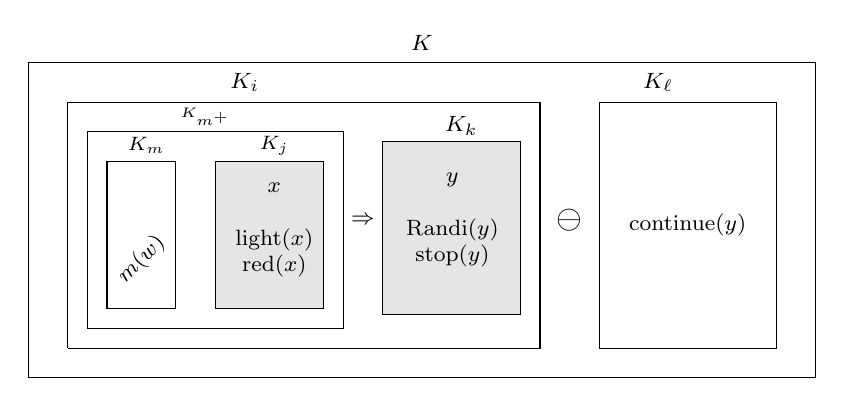
\begin{tikzpicture}\footnotesize
\draw (0,0) -- (10,0) -- (10,4) -- (0,4) -- (0,0);%Kbox
\draw (.5,.375) -- (6.5,.375) -- (6.5,3.5) -- (.5,3.5) -- (.5,.375);%Ki box
\draw (.75,.625) -- (4,.625) -- (4,3.125) -- (.75,3.125) -- (.75,.625);%Km+ box
\draw (1,.875) -- (1.875,.875) -- (1.875,2.75) -- (1,2.75) -- (1,.875);%Km box
\node[align=center,rotate=45] at (1.4375,1.5) {$m(w)$};%Kmtext
\draw[fill=gray!20] (2.375,.875) -- (3.75,.875) -- (3.75,2.75) -- (2.375,2.75) -- (2.375,.875);%Kj box
\node[align=center] at (3.125,1.875) {$x$\\\\ light($x$)\\red($x$)};%Kjtext
\draw[fill=gray!20] (4.5,.8) -- (6.25,.8) -- (6.25,3) -- (4.5,3) -- (4.5,.8);%Kk box
\node[align=center] at (5.3875,2) {$y$\\\\ Randi($y$)\\stop($y$)};%Kk txt
\draw (7.25,.375) -- (9.5,0.375) -- (9.5,3.5) -- (7.25,3.5) -- (7.25,0.375);%KL
\node[align=center] at (8.375,2) {\\ continue($y$)}; %\\$ z=y $		
\node[align=center] at (2.125,1.875) {{$\Cap$}}; %conditional op
\node[align=center] at (6.875,2) {{\large$\ominus$}}; %otherwise op
\node[align=center] at (4.25,2) {{$\boldsymbol\Rightarrow$}}; %cons op
%%
\node[align=center] at (5,4.25) {$ K $}	;
\node[align=center] at (2.75,3.75) {$\boldsymbol{K_i} $};
\node[align=center] at (2.25,3.3125) {{\tiny$\boldsymbol{ K_{m^+}} $}};
\node[align=center] at (1.5,2.95) {{\scriptsize$ \boldsymbol{K_m} $}};
\node[align=center] at (3.125,2.95) {{\scriptsize$ K_{j} $}};
\node[align=center] at (5.5,3.2) {$ K_k $};
\node[align=center] at (8,3.75) {$ K_\ell $};\\
\end{tikzpicture}
\-\\\vspace{1pt}
Where the following satisfaction conditions hold:
\begin{itemize}
  	\item \, $C_K = \{K_i\underset{m,o}{\ominus} K_\ell\}$
	\item \, $C_{K_i} =\{ K_j\, \underset{m,o}{\square}\, K_k\} = \{K_{m^+}\Rightarrow K_k	\}$
	%&C_{K_{m^+}}=\{\}\\
	\item  $C_{K_j} = \{\text{light}(x),\,\text{red}(x)\}$
	\item  $C_{K_k} = \{\text{Randi}(y), \text{stop}(y)\}$
	\item  $C_{K_\ell} = \{\text{continue}(y)\}$
	\item  $C_{K_m} = \{c\mid\langle w',f\rangle\Vdash c\} \text{ where } w'\in\underset{deo(w)}{\textsc{best}}\big(\cap\underset{\textsc{circ}}{m(w)}\big)$
	\item  $C_{K_{m^+}} = \{K_m\Cap K_j\} = \{c\mid\langle w''\!,f\rangle\Vdash c\} $
%where $w''\in\underset{deo(w)}{\textsc{best}}\big(\cap\big(\underset{\textsc{circ}}{m(w)}\cup\{w'''\mid\langle w'''\!\!,f\rangle\vDash K_j\}\big)\big) $
\end{itemize}
\a DRS illustration spelling out accommodation of the antecedent proposition $ (K_{i_{\text{sub}}}) $ (compare to \S \ref{sec:proposal}, esp. exx. \ref{redlight-Ki} \& \ref{antec-skel}):\\
\drs{~}{\hfill\xdrs{~~~$K_i$}\\$ \neg $\xdrs{~~~$ K_{m^+} $}$\square$\xdrs{~~~$ K_\ell $}}
\xe%

%\textcolor{red}{Josh: I changed a couple of the satisfaction conditions from what you had originally. Do you notice any issues there? }\textcolor{violet}{i don't thiiiink i do? do you remember what they were?}

With the satisfaction conditions we introduced above, we can construct the truth-conditions that will verify the matrix DRS $ K $: 

\pex \textit{Satisfaction conditions for \blastx:}
\a\uline{Simplex conditions:}\\ 
The DRSs $ K_j,K_k,K_\ell $ all contain only atomic conditions.\\ Each of these DRSs is verified iff there is some world-assignment pair $ \langle w,f\rangle $ which satisfies all of their respective conditions.\\
\begin{itemize}
	\item  $\langle w,f\rangle \vDash K_j \leftrightarrow \langle w,f\rangle \Vdash \text{red.light}(y) \leftrightarrow f(y)\in\Sem[w]{red.light}$\\
	\item   $\langle w,f\rangle \vDash K_k \leftrightarrow \langle w,f\rangle \Vdash \text{Randi}(y)\wedge \text{stop}(y) \leftrightarrow f(y)\in\Sem[w]{Randi}\cap\Sem[w]{stop}$\\
	\item   $\langle w,f\rangle \vDash K_\ell \leftrightarrow \langle w,f\rangle \Vdash \text{continue}(y) \leftrightarrow f(y)\in\Sem[w]{continue}$
\end{itemize}
\a \uline{The antecedent to \textit{otherwise} $ C_{K_i} $:}\\
The antecedent $ K_i $ is verified iff some world-assignment pair $ \langle w,f\rangle $ satisfies the (complex) condition $ K_j\,\square\,K_k $ :\\ 
%
$\langle w,f\rangle\Vdash (K_j\underset{m,o}{\square} K_k )\leftrightarrow \\
  	\forall w',g\big[g{\scriptscriptstyle\langle X_{K_j}\rangle}f \wedge w'\in\underset{tel(w)}{\textsc{best}}\big(\bigcap\big(\underset{\textsc{circ}}{m(w)}\cup\{w''\mid\langle w'',g\rangle\vDash K_j\}\big)\big) \to\\
	\hspace*{2.7em} \exists g''[g''{\scriptscriptstyle\langle X_{K_k}\rangle}g \wedge \langle w',g''\rangle\vDash K_k]\big]$\\[1em]
%
That is: $ \langle w,f\rangle\vDash K_i $ iff for all $ w' $ in a circumstantial modal base $ \underset{\textsc{circ}}{m(w)} $ that best conform to a teleological ordering source $ o_{tel}(w) $: if there is some assignment $g'$ that verifies $ K_j $ in $w'$, then there is some assignment $ g'' $ that verifies $ K_k $  in $w'$.
\a \uline{The matrix condition $ C_K $:}\\
A world-assignment pair $\langle  w,f \rangle$ verifies the entire DRS $ K $ iff it satisfies the (complex) condition $ K_i\ominus K_\ell $ : 
\label{Ck}\\
%
$\langle w,f\rangle \Vdash(K_i\underset{m',o'}{\ominus} K_\ell)\leftrightarrow\exists g[g{\scriptscriptstyle\langle X_{K_i}\rangle}f\wedge\langle w,g\rangle\vDash K_i] 
\;\wedge\\
\forall w',g'[g'{\scriptscriptstyle\langle X_{K_i}\rangle}f\wedge w'\in\underset{tel(w)}{\textsc{best}}\Big(\bigcap\big(\underset{\textsc{circ}}{m'(w)}\cup\{w''\mid\langle w'',g'\rangle\vDash(\neg K_{i_{\text{sub}}})\}\big)\Big) \to\\
	\hspace*{2.85em} \exists g''(g''{\scriptscriptstyle\langle X_{K_\ell}\rangle}g'\wedge \langle w',g''\rangle\vDash K_\ell)]$\\[1em]
%\end{multline*}
That is: $ \langle w,f\rangle\vDash K $ iff:
\begin{itemize}
	\item \; There is some assignment $ g $ that verifies $ K_i $ and
	\item \; If those worlds $ w' $ in a circumstantial modal base $\underset{\textsc{circ}}{m(w)}$ that best conform to a teleological ordering source (likely one that contains Randi's desires to both get where she needs to be and to be an upstanding road user) \textbf{verify the negation of} $ \boldsymbol{ K_{m^+}} $ (the antecedent to \textit{otherwise}, accommodated due to the processes described in \S\ref{sec:qud}), then there'll be some assignment $ g'' $ that verifies $ K_\ell $ in $w'$.
\end{itemize}
%
\xe
%\textcolor{red}{Josh, please add descriptions of these formulas (at least in a and b) in words. This is really hard to follow. Specifically, define $O_{tel}$, $m_{circ}$. What does this complex condition require?}

Notably, $ y $ is an unbound variable in its local DRS --- however, because $ K_i\leqslant K_\ell $, $ K_\ell $  has access to the local domain of this DRS $ (A_{K_\ell}\supseteq X_{K_{i}}) $. As a result, the assignment function ($ g'' $ in \ref{Ck} above) is able to assign to $ y $ an individual introduced earlier in the discourse (namely `Randi').
 We see, then, that our analysis is able to correctly model an \textit{otherwise} statement, making crucial use of the notion of modal subordination and other tools that foreground discourse dynamics to provide the truth conditions for the sentence. 
 
 
 
 
 
